%!TEX root = main.tex

\documentclass[../main.tex]{subfiles}

\begin{document}

\chapter{Description of Slide Guitar Synthesis Model}
\label{ch:three}
In this section, we introduce the synthesis model which was developed based on the theory from Chapter~\ref{ch:background}. After the model has been introduced, there will be an exploration of the limitations of the design and the theoretical reasons behind them.

\section{Introduction of Architecture}
The slide guitar synthesizer developed in this thesis is heavily influenced by the model introduced in \citetwo{pakarinen_virtual_2008} and \citetwo{puputti_real-time_2010}. Modifications were made during development and they will be explained as they are introduced. The model consists of three main components: the Control Signal Processor (CSP), the Contact Sound Generator (CSG) and a String Digital Waveguide (DWG) model. The Control Signal Processor's main job is to compute derived parameters from the control signal which are used to control the other two components. The Contact Sound Generator produces the sound corresponding to the slide and string surface interactions. The String Digital Waveguide synthesizes the sounds associated with the transverse vibrations of a plucked-string of time-varying length. Audio examples will also be provided in an effort to facilitate an aurally intuitive understanding of the model by bridging the gap between the theoretical design and the perceptual/experiential end result.

\subsection{Diagram Conventions}
The following conventions will be adhered to in this section's diagrams. This was done to improve clarity and reduce ambiguity as compared to the diagrams from the original papers \citetwo{pakarinen_virtual_2008} and \citetwo{puputti_real-time_2010}. Figure~\ref{fig:slide_synth} serves an illustrative example.

In synthesis systems, signals can functionally divided into two different categories: control signals and audio signals. This is illustrated by the use of dashed lines for control signals, and the use solid lines for audio signals. It is also common that the control signals are run at a sampling rate which is lower than or equal to the audio rate. This has been represented by the use of different indices for the time-index. $[m]$ represents a signal at the control rate while $[n]$ represents a signal at the audio rate. It is possible to have a control signal at the audio rate as is illustrated by $L[n]$ in Fig.~\ref{fig:slide_synth}.

\subsection{Single String Slide Synthesizer}

\begin{figure}[h]
    \centering
    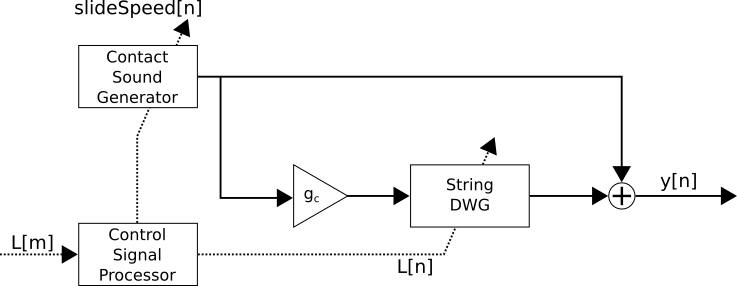
\includegraphics[scale=.65]{./images/diagrams/slideSynth.png}
    \caption{The high-level architecture for a single string slide synthesizer.}
    \label{fig:slide_synth}
\end{figure}

The highest-level component of the synthesis system is depicted in Fig.~\ref{fig:slide_synth}. This is a synthesizer for a single string where the pitch is controlled by a slide. Similar to the model introduced in Chapter 2, this consists of a module which represents a variable length string digital waveguide as well as a contact sound generator for the string/slide surface interactions. 

The first new addition is a gain block which controls the coupling between the longitudinal motion of the slide and the transverse vibrations of the string. The CSG model only considers longitudinal slide motion in its algorithm. The coupling phenomena was experimentally observed on a per string basis, as will be shown in Sec.~\ref{sec:couplingMeasurements}.

The Control Signal Processor is another new block which will be more carefully detailed in the next section. It was placed at the highest possible layer in the architecture. This placement improves computational efficiency by removing redundant computations in lower-levels as well as ensures all the constituent processing and synthesis objects are operating on a common set of control signal values.

\subsection{Control Signal Processor}
\label{subsec:Ch3ControlSignalProcessor}

\begin{figure}[h]
    \centering
    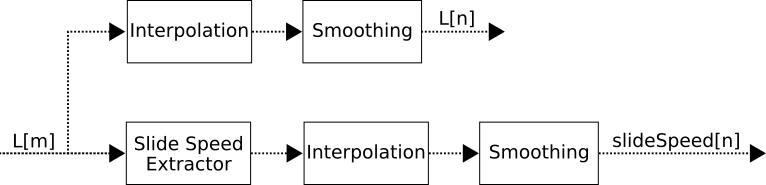
\includegraphics[scale=.65]{./images/diagrams/controlSignalProcessor.png}
    \caption{The signal-flow diagram for control signal processor block.}
    \label{fig:CSP}
\end{figure}

Figure~\ref{fig:CSP} illustrates the internals of how the Control Signal Processor operates. Its input signal is the relative length control signal at control rate. Its output signals are the slide speed as well as relative length signal at audio rate. The purpose of this block is to extract the slide speed signal as well as change the control rate signals to audio rate.

The interpolation is linear and upsamples the control rate signals to the audio rate.. This allows more gradual changes between control signal values to be seen by the audio rate objects as this is beneficial for preventing unwanted artifacts (e.g, transients). Supposing that $R$ represents the ratio between the control rate and audio rate, then for each one control-sample, $R-1$ audio samples are calculated via the interpolation. In the case where the audio rate is 48,000 kHz and the control rate is 1 kHz then $R = \frac{48,000}{1,000} = 48$ and 47 additional samples would be calculated.

The smoothing helps eliminate any discontinuities which may be present in the interpolated signal. It is implemented via a 10-point moving window averager.

\subsubsection{Slide Speed Extractor}

\begin{figure}[h]
    \centering
    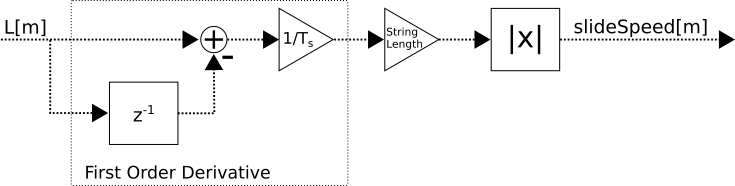
\includegraphics[scale=.5]{./images/diagrams/slideSpeedExtractor.png}
    \caption{The signal-flow diagram for slide speed extractor block.}
    \label{fig:SSE}
\end{figure}

Figure~\ref{fig:SSE} shows a signal-flow diagram for the slide speed extractor. This is similar to the model introduced in \citetwo{pakarinen_virtual_2008} with some refinements for precision and clarity. Functionally it operates in the following manner. The first step is to take a difference between two consecutive samples and divide this by the sampling period. This is an approximation of the first derivative and has units of $\frac{\Delta \text{relative length}}{\text{sec}}$. The next step is to convert this from a relative length to an absolute length through multiplication by the length of a string in meters. This produces the absolute slide velocity in $\frac{\text{meters}}{\text{sec}}$. From there, the absolute value is taken to convert the velocity to a speed. Speed is used here as the Contact Sound Generator is agnostic to the direction the slide moves and is the only synthesis object which is concerned with slide speed.

\subsection{String DWG}

\begin{figure}[h]
    \centering
    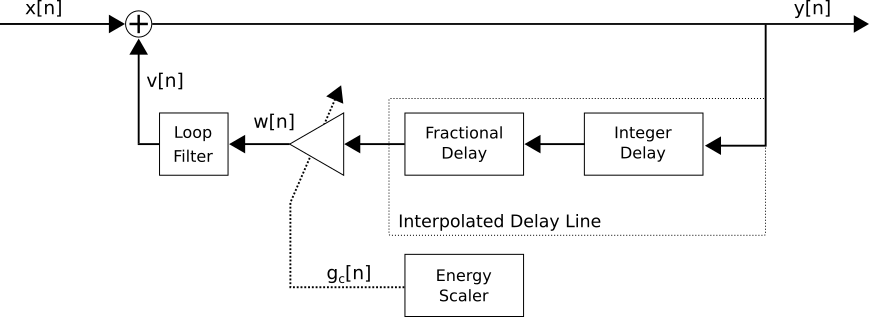
\includegraphics[scale=.5]{./images/diagrams/stringDWG.png}
    \caption{The signal-flow diagram for the time-varying string DWG. $L[n]$ is not depicted as every object consumes it in some fashion.}
    \label{fig:stringDWG}
\end{figure}

Figure~\ref{fig:stringDWG} illustrates the string digital wave guide model. The model itself does not differ from the original as described in \citetwo{pakarinen_virtual_2008}. However, the diagram here differs in an attempt to improve clarity as compared to the original. $L[n]$ is not depicted as all the signal processing blocks shown rely on this in some manner. Additionally, there have been intermediate signals introduced ($v[n]$ and $w[n]$) as they were beneficial in developing the implementation.

\subsubsection{Energy Scaler}
\label{subsec:Ch3EnergyScaler}
It was necessary to slightly rearrange the original energy scaling equation (Eq.~\ref{eq:energyScaler}) from Chapter~\ref{ch:background} to indicate the time-varying aspect of $g_c[n]$ and help facilitate its computation. The implementation computes the gain coefficient using the following expression:
\begin{equation}
    \label{eq:energyScalingImplementation}
    g_c[n] = \sqrt{1-\Delta x[n]}
\end{equation}
where $\Delta x[n]$ is the difference in the length of the digital waveguide between two successive samples and $g_c[n]$ is the coefficient which performs the scaling. Figure~\ref{fig:energyScaler} illustrates the signal-flow diagram of the energy scaler object which computes this gain value.
\begin{figure}[h]
    \centering
    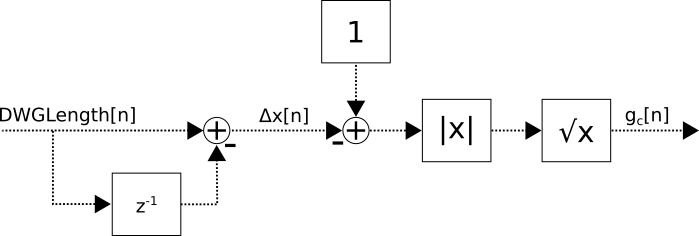
\includegraphics[scale=.5]{./images/diagrams/energyScaler.png}
    \caption{The signal-flow diagram for the energy scaler block implementing Eq.~\ref{eq:energyScalingImplementation}.}
    \label{fig:energyScaler}
\end{figure}

\subsubsection{Loop Filter}
The loop filter is single-pole and simulates the losses associated with string vibration. It has been described previously in Sec.~\ref{sec:Ch2LoopFilter}. There is no novelty in its implementation due to the standardization of the single-pole design.

\subsection{Contact Sound Generator}
Two varieties of the Contact Sound Generator exist, corresponding to the two different varieties of strings which exist. First, the unwound approach will described. It is the simpler of the two models and describes the sound produced when the slide interacts with the smooth surface of an unwound string. Subsequently, the more complex wound string variant will be examined in detail.

\subsubsection{Unwound Strings}
Figure~\ref{fig:CSG_unwound} shows the signal-flow diagram for the unwound Contact Sound Generator. The unwound strings have a substantially simpler algorithm as the sound is generated from two smooth surfaces interacting with each other. It is more akin to a friction sound generator as opposed to an impact sound, which matches the interaction between the surfaces. This contact noise can easily be modeled by low-pass filtered white noise which has its amplitude scaled by the slide's speed. A user-tunable parameter for the overall contact sound level is placed at the end of the chain. This does not differ from the original design described in \citetwo{pakarinen_virtual_2008} and implemented in \citetwo{puputti_real-time_2010}.

\begin{figure}[h]
    \centering
    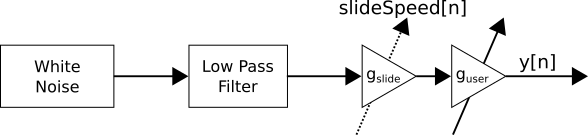
\includegraphics[scale=.5]{./images/diagrams/CSG_unwound.png}
    \caption{The signal-flow diagram for unwound Contact Sound Generator block.}
    \label{fig:CSG_unwound}
\end{figure}

\subsubsection{Wound Strings}
\label{subsec:WoundString}
Figure~\ref{fig:CSG_wound} illustrates the signal-flow diagram for the wound string Contact Sound Generator. The core functionality does not differ from the module which was suggested in \citetwo{pakarinen_virtual_2008} in that it uses the speed of the slide to generate a sound containing a time-varying harmonic component ($v_2[n]$) and a static component due to the longitudinal modes ($v_1[n]$). It does, however,  differ substantially from the implementation in \citetwo{puputti_real-time_2010}. Additionally, variations of different components have been implemented to experiment with different timbres as indicated by the more general ``Noise Pulse/Burst Source" and ``Harmonic Accentuator" blocks.

The longitudinal mode filter remains a 4th-order IIR using the same coefficients as specified in the original paper \citetwo{pakarinen_virtual_2008}. There is also the linked pair of gain blocks which allows the balance between the static and harmonic components to be varied. The last gain block, $g_{user}$, allows the overall sound level to be specified (as in the unwound implementation).

The first step in the wound Contact Sound Generator is to convert the incoming $slideSpeed[n]$ to a frequency based on the linear density of string windings associated with the string. This $f_c[n]$ represents the rate at which the slide-to-winding collisions occur. Its name comes from the fact that the control signal is used to control the centre frequency of the resonator filter in the harmonic accentuator which is tuned to the fundamental frequency of the generated contact sound. The $n_w$ parameter is stored here to keep all the information specific to the string's physical properties in a single location.

\begin{figure}[h]
    \centering
    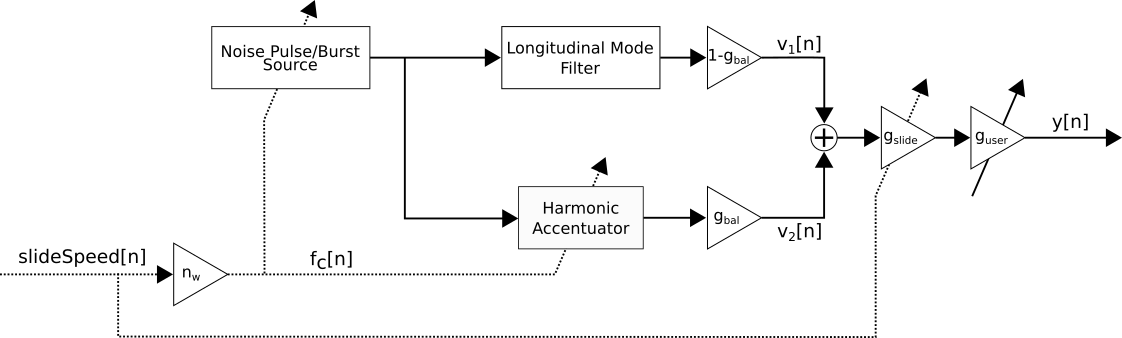
\includegraphics[scale=.5]{./images/diagrams/CSG_wound.png}
    \caption{The signal-flow diagram for wound CSG block.}
    \label{fig:CSG_wound}
\end{figure}

\paragraph{Noise Source}
Two variations for noise sources were developed through the course of this thesis. The first is conceptually not different from what was described in \citetwo{pakarinen_virtual_2008}, however in implementation it differs significantly from the version in \citetwo{puputti_real-time_2010}. The second is more akin to what was introduced in  the guqin model in \citetwo{penttinen_model-based_2006}.

\subparagraph{Noise Pulse Train}
\label{para:NPT}
Figure~\ref{fig:NoisePulseTrain} illustrates the first variation on a noise source. It consists of absolute-valued white noise which has an amplitude envelope applied to it. This amplitude envelope is generated by an impulse train which is fed into a one-pole filter. The firing rate of the impulse train is controlled by the $f_c[n]$ signal which mimics the generation of impulses from the slide hitting windings as it moves. The decay rate of the impulse response of the one-pole filter is controlled by the $T_{60}$ value measured for each string (which will be elaborated upon in Sec.~\ref{sec:DecayRateMeasurement}). The use of a one-pole filter allows the generated impulses to stack on top of each other and also benefits from being extremely computationally efficient. A DC blocker was added to remove the DC component introduced by the absolute-value function. Without applying an absolute value, the signal remains too noise-like to be harmonic.

\begin{figure}[h]
    \centering
    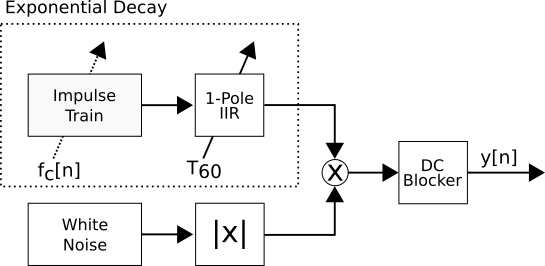
\includegraphics[scale=.5]{./images/diagrams/NoisePulseTrain.png}
    \caption{The signal-flow diagram for the Noise Pulse Train.}
    \label{fig:NoisePulseTrain}
\end{figure}

\subparagraph{Noise Burst Generator}
\label{subpara:Ch3NBG}
Figure~\ref{fig:NoiseBurstGen} illustrates the second variation of a noise source. This attempts to combine the method used in the guqin model \citetwo{penttinen_model-based_2006} with more string specific characteristics as the slide guitar model \citetwo{pakarinen_virtual_2008}. White noise is multiplied by an amplitude envelope as before. However, in this variation the output of the one-pole filter is hard-clipped to a value of 1. In areas of a slow slide movement the output is similar to the noise pulse train, however as the slide speed increases and more windings are struck, the signal transitions into white noise and the harmonic component is lost (subject to the value of $T_{60}$). The one-pole also ensures that the starting and stopping of the noise will be more ``natural" with the addition of the decay rate. Otherwise, the envelope would be a pure step-function and not allow more gradual changes. This component was developed as the more noise-like characteristics of its output would perform better with the Harmonic Resonantor Bank (described next) and to provide a second approach for comparison with the Noise Pulse Train.

\begin{figure}[h]
    \centering
    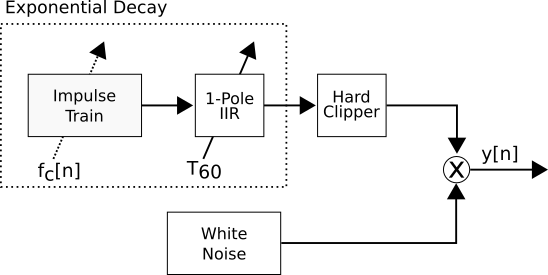
\includegraphics[scale=.5]{./images/diagrams/NoiseBurstGen.png}
    \caption{The signal-flow diagram for the Noise Burst Generator.}
    \label{fig:NoiseBurstGen}
\end{figure}

\subparagraph{Impulse Train}
\label{subpar:Ch3ImpulseTrain}
Both the Noise Pusle Train and Noise Burst Generator have a common component in the Impulse Train. The Impulse Train object outputs a discrete-impulse signal at a specified period in samples. Internally, it counts the number of samples which have passed until it is time to generate a new impulse. The period, in samples, is computed using the following equation:

\begin{equation}
    period = \text{round}\left(\frac{F_s}{f_c[n]}\right)
    \label{eq:f_cQuantization}
\end{equation}

\paragraph{Harmonic Accentuation}
\label{para:Ch3HarmonicAccentuation}
Two variations for accentuating and generating the harmonics of the wound contact sounds were investigated. The first method is the same as what is described in \citetwo{pakarinen_virtual_2008}, while the second is more akin to the method proposed for the guquin model \citetwo{penttinen_model-based_2006}. These methods provide more control over the strength and number of harmonics as compared to what is available based purely on the parameters of the noise sources.

\subparagraph{Reso + Tanh}
\label{subpar:Ch3Reso+Tanh}
The first method is a second-order resonator in series with a hyperbolic tangent function as illustrated in Fig.~\ref{fig:ResoTanh}. The second-order resonator has its center frequency controlled by $f_c[n]$ and its $r = .99$. This configuration allows the filter to isolate the fundamental of the input signal. Assuming the input signal has a fundamental, the $\tanh$ function will introduce harmonics. The number of harmonics is controlled by the scaling factor $g$ ahead of it in the signal chain. This provides an extremely computationally efficient approach to generating the harmonics, at the expense of more fine-tuned control over the number and strength of each individual harmonic.

\begin{figure}[h]
    \centering
    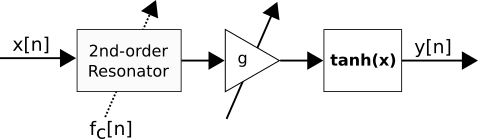
\includegraphics[scale=.5]{./images/diagrams/ResoTanh.png}
    \caption{The signal-flow diagram for the Reso + Tanh waveshaper.}
    \label{fig:ResoTanh}
\end{figure}

\subparagraph{Harmonic Resonator Bank}
The second approach is illustrated in Fig.~\ref{fig:HRB}. This method is more computationally expensive, but provides much more control over the strength, number and location of the different harmonics. Additionally, it works with input sources that are both noisy and harmonic. It consists of a set of parallel second-order resonators whose centre frequencies are all harmonically linked to each other. At the output of each resonator is a tuneable gain coefficient to control the strength of the isolated harmonic. Six harmonics were chosen based on the spectrograms in \citetwo{pakarinen_virtual_2008}, however the object itself supports an arbitrary number.

\begin{figure}[h]
    \centering
    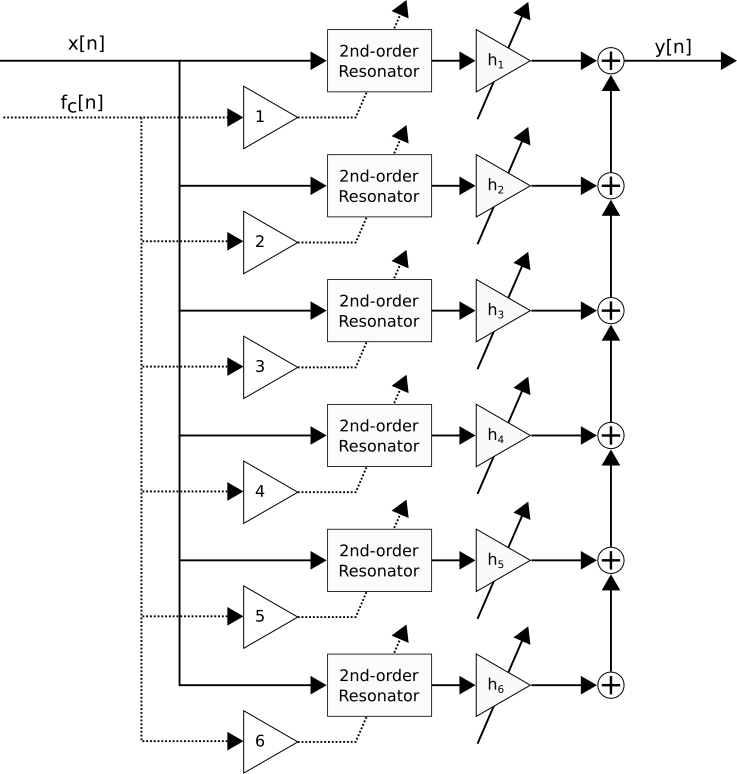
\includegraphics[scale=.5]{./images/diagrams/HarmonicResonatorBank.png}
    \caption{The signal-flow diagram for the Harmonic Resonator Bank.}
    \label{fig:HRB}
\end{figure}

\section{Limitations of Model}
\subsection{Minimum Relative String Length}
\label{sec:MinL}
Although not explicitly mentioned in the source literature, there is a limit imposed on the minimum value $L[n]$ can take based on the magnitude response of the Loop Filter. The limits of this can be deduced from the original figures which describe the loop coefficients in \citetwo{valimaki_development_1998}.

\citetwo{valimaki_development_1998} describe the method by which the polynomials used to generate the Loop Filter's $a$ and $g$ values are derived from recordings of a professional guitar player playing several tones on all frets of every string in an anechoic chamber. Unfortunately, there is no standardization between guitar manufacturers as to the appropriate number of frets for a guitar. Common values are 21, 22 and 24 \citetwo{erlewine_how_2001}. With knowledge of the model used by the player in the aforementioned paper, one could look up the number of frets on a manufacturer's website. However, this information is not available in the source material. By observing the Loop Filter's magnitude response as it changes based on $L[n]$ and reverse-engineering the values in the original graphs it is possible to reasonably conclude the recordings used to derive the polynomials stopped at the 19th fret.

Figure~\ref{fig:originalLoopGain} from the Sec.~\ref{sec:Ch2LoopFilter} illustrates the loop gain $g$ across different frequencies for the high E string. By combining Eq.~\ref{eq:F_L} and Eq.~\ref{eq:fretNumber}, it is possible to generate the fundamental frequencies associated with each fret on the string. Table~\ref{tab:eStringFrets} illustrates this for a selection of frets on the high E string. From this table we can see that the most likely candidate for the upper-most fret used by the player in the recordings is the 19th fret based on the upper limit for the x-axis in Fig.~\ref{fig:originalLoopGain}.

\begin{table}[h]
\centering
\begin{tabular}{|c| c|} 
 \hline
 \textbf{Fret \#} & \textbf{Fundamental} \emph(Hz) \\ [0.5ex] 
 \hline
 0 & 329.63\\
 18 & 932.33\\
 19 & 987.77\\
 20 & 1046.5\\
 \hline
\end{tabular}
\caption{The calculated fundamental frequencies for a selection of frets on the high E string.}
\label{tab:eStringFrets}
\end{table}

Figure~\ref{fig:UnstableLoopString1} and Fig.~\ref{fig:UnstableLoopString4} illustrate the magnitude response for string \#1 (the high E) and string \#4 (the D string) across a variety of upper frets to show how they transition in this range. The general pattern is that each filter gradually shifts from a low-pass type response to more of a high-pass type response. Eventually the gain goes above 0 dB as well. This occurs at fret 24 for the high E string and fret 22 for the D string. Given the placement of the filter in the feedback loop of the digital waveguide, a positive gain value results in an unstable state. Based on the data presented in Fig.~\ref{fig:originalLoopGain} and Table~\ref{tab:eStringFrets}, the Loop Filter has clearly gone beyond the range of its original design under these conditions. However, this would be considered a limitation as in slide playing the slide often goes beyond the 24th fret. Even before reaching the point of positive amplification, the deviation from a low-pass filter causes the harmonics to decay in a manner which is not consistent with physical reality and is considered a limitation. 

\begin{figure}[h]
    \centering
    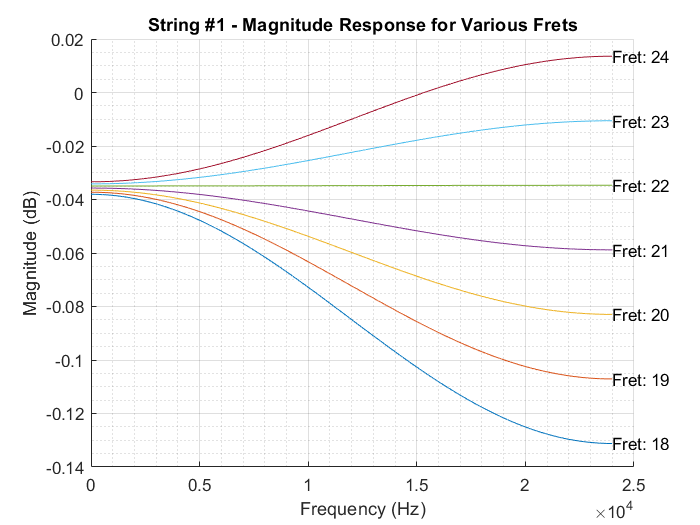
\includegraphics[scale=.65]{./images/plots/Unstable Loop Filter - String 1.png}
    \caption{The loop filter magnitude response for the high E string at a variety of frets to illustrate its transition to a positive gain in the upper frequencies.}
    \label{fig:UnstableLoopString1}
\end{figure}

\begin{figure}[h]
    \centering
    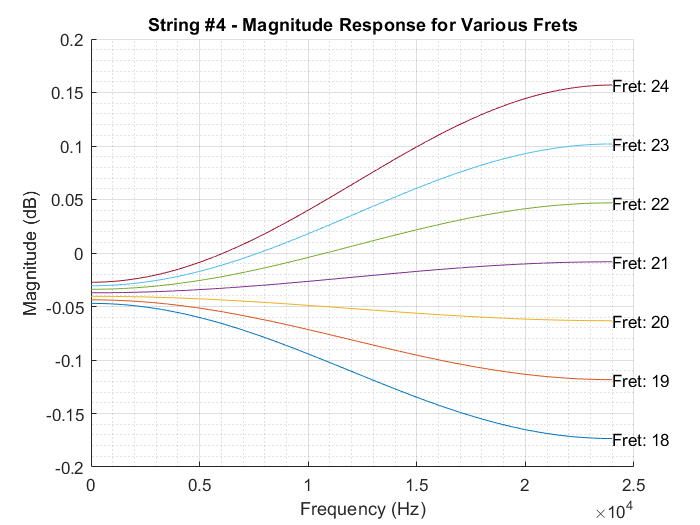
\includegraphics[scale=.65]{./images/plots/Unstable Loop Filter - String 4.png}
    \caption{The loop filter magnitude response for the D string at a variety of frets to illustrate its transition to a positive gain in the upper frequencies.}
    \label{fig:UnstableLoopString4}
\end{figure}

\clearpage

\subsection{Non-constant Phase Delay of Filters}
As mentioned in Sec.~\ref{subsec:Ch2DigitalFilters}, the phase delay is a function of frequency indicating the time-delay, in samples, each frequency component experiences. The phase delay is physically correlated with the wave speed and in order to have the most accurate tuning, both these functions would be constant across the spectrum. However, a constant function is not always the most physically accurate.

Both the loop filter as well as the interpolation filter illustrate non-constant phase delays. This is shown in Fig.~\ref{fig:LagrangePhaseDelays} and Fig.~\ref{fig:Str5PhaseDelays}. The loop filter illustrates this as it is an IIR filter. This is inherent in their design \citetwo{oppenheim_discrete-time_2010}. The interpolation filter is an FIR and under certain circumstances it can actually illustrate a constant delay (when the order is even and the fractional delay is 0.5) \citetwo{laakso_splitting_1996}.

Many strings in reality exhibit some form of stiffness which results in different wave speeds for different frequencies. This dispersion results in the observed overtones being slightly different than what an idealized string model would predict. The nature of a non-constant phase delay is similar to this, however it is more of an uncontrolled artifact here as opposed to intentional modeling. Although the values are small here and likely do not have an impact, they clearly vary with the relative length signal and ultimately will affect the accuracy of the tuning from a computational standpoint. Given that this model was originally designed to be played in real-time, this can easily be compensated for via ``on-the-fly" tuning by ear if need be.

\begin{figure}[h]
    \centering
    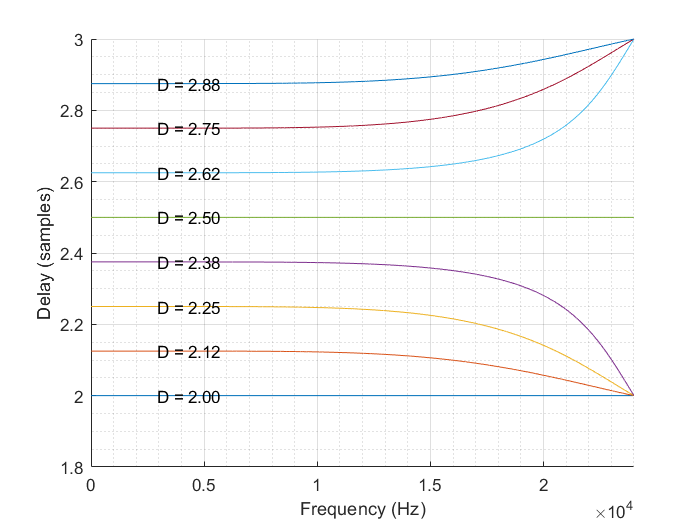
\includegraphics[scale=.65]{./images/plots/LagrangePhaseDelays.png}
    \caption{The phase delays for Lagrange interpolating filters with order = 5 at various delay values.}
    \label{fig:LagrangePhaseDelays}
\end{figure}

\begin{figure}[h]
    \centering
    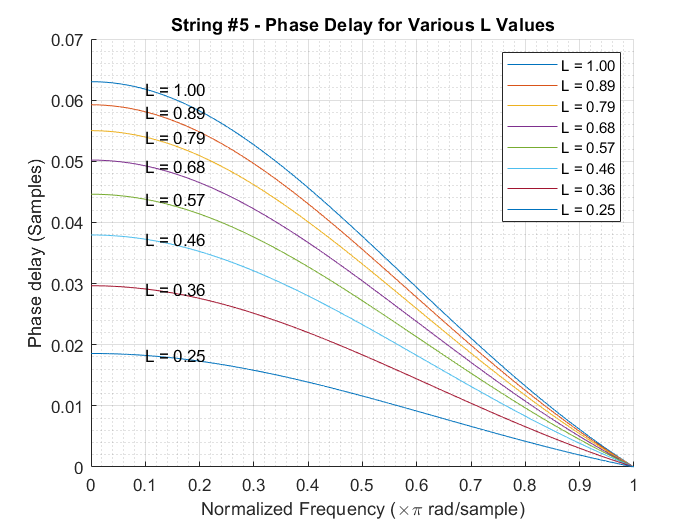
\includegraphics[scale=.65]{./images/plots/String 5 - Phase Delays.png}
    \caption{The phase delay for A string's loop filter at various relative lengths.}
    \label{fig:Str5PhaseDelays}
\end{figure}

\subsection{Impulse Train Quantization}
The Impulse Train is limited to integer period values as its implementation is based on counting individual samples. Given the reciprocal nature between frequency and period, this ends up quantizing the frequencies which the Impulse Train effectively operates. The quantization is worse at higher frequencies as compared to lower ones for a selected $F_s$ and can be mitigated by increasing $F_s$ as this correspondingly decreases $T_s$ and increases the time-resolution of the system. Similar effects have been noted in \citetwo{jaffe_extensions_1983} in regards to tuning. One possible approach to mitigating this is by interpolating the impulse train signal.

Figure~\ref{fig:f_cQuantized} illustrates the effects of the rounding on the range of possible frequencies for a sampling rate of 48 kHz. The effects on an $f_c[n]$ sweep matching the trajectory a slide might generate as well as the corresponding harmonics are shown in Fig.~\ref{fig:f_cSweepQuantized}. The effects can be seen in the output of the Noise Pulse Train (see Sec.~\ref{para:NPT}) object to the parabolic $f_c[n]$ sweep shown in Fig.~\ref{fig:f_cQuantizedSpectrum} and can be heard in \emph{f\_cSweepQuantization-NPT.wav}\footnote{Sound examples can be found: \url{https://github.com/dgsmith1988/Masters-Thesis/tree/main/Sound\%20Examples}}. The Noise Pulse Train object uses a $T_{60}$ value tuned to generate harmonics as opposed to noise. The effects of this parameter will be detailed more fully in the Sound Design and Parametrization chapter.

\begin{figure}[h]
    \centering
    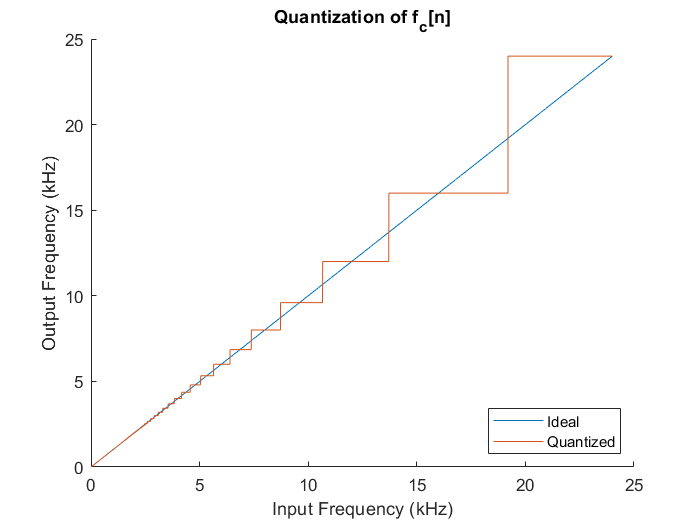
\includegraphics[scale=.65]{./images/plots/f_cQuantization.png}
    \caption{The quantization effects from Eq.~\ref{eq:f_cQuantization} for a sampling rate of 48 kHz.}
    \label{fig:f_cQuantized}
\end{figure}

\begin{figure}[h!]
    \centering
    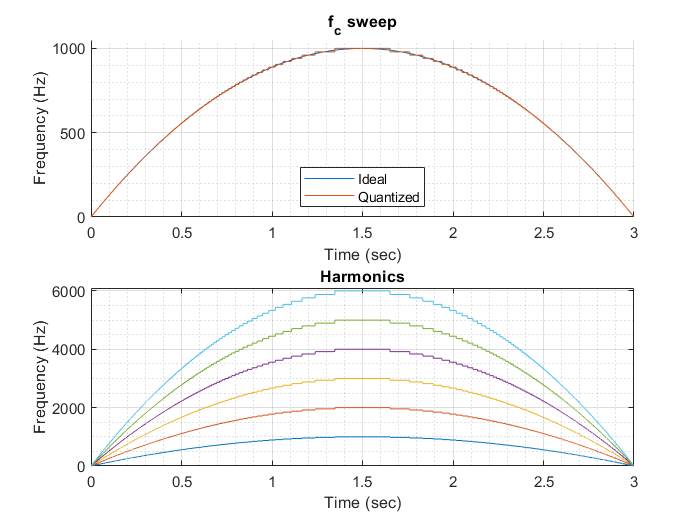
\includegraphics[scale=.65]{./images/plots/f_cSweepQuantized.png}
    \caption{The quantization effects for a parabolic sweep and the corresponding impact on the first six harmonics. Note how the effects are amplified in the higher harmonics.}
    \label{fig:f_cSweepQuantized}
\end{figure}

\clearpage

\setcounter{footnote}{0} 

\begin{figure}[h!]
    \centering
    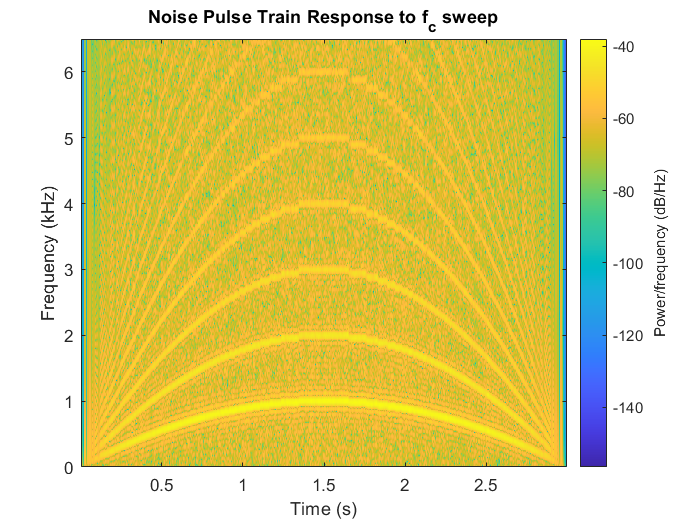
\includegraphics[scale=.50]{./images/plots/f_cSweepNPT.png}
    \caption[Caption for quantized spectrogram]{Spectrogram of the output of the Noise Pulse Train in response to the parabolic $f_c[n]$ sweep from Fig.~\ref{fig:f_cSweepQuantized}. The plot has been zoomed in to emphasize the effects on the first six harmonics. The output can be heard in \emph{f\_cSweepQuantization-NPT.wav}\footnotemark.}
    \label{fig:f_cQuantizedSpectrum}
\end{figure}

\footnotetext{Sound examples can be found: \url{https://github.com/dgsmith1988/Masters-Thesis/tree/main/Sound\%20Examples}}

\subsection{Nyquist Rate Implications}
A limitation in all digital systems exists as an upper limit on the frequencies which can be represented. This is referred to as the Nyquist Rate and is equal to $\frac{F_s}{2}$. With regard to the slide guitar synthesis model, the largest implication of the Nyquist Rate is an upper limit on the harmonics which can be represented in the system. From a physical standpoint, these harmonics above this Nyquist rate would exist. In actual practice, these upper harmonics are very weakly stimulated and contribute very little to the actual perception of the sound as the human range of hearing is limited to approximately 20 kHz \citetwo{plack_sense_2018}. Using a sampling rate of 48 kHz results in a Nyquist Rate of 24 kHz, and taking into account the limits of human hearing the physical inaccuracies are acceptable from the standpoint of a sound synthesis algorithm.
\end{document}